\documentclass{article}

\usepackage{Engineering}

% === TEXT ===
\title{\textbf{Basis of Sustainable Environmental Systems \\ HSLU, Semester 3}}
\author{Matteo Frongillo}

\begin{document}

\maketitle
\tableofcontents
\pagebreak

\part{TODO ops}
i'll do it later don't worry

\newpage
\part{Separation techniques}
\section{A bit of chem again}
\subsection{Solutions key terms}
\begin{itemize}
    \item \textbf{Solvent}: the substance that dissolves another substance 
    \item \textbf{Solute}: the substance that is dissolved in a solvent
    \item \textbf{Solution}: it's a homogeneous mixture of two or more substances
\end{itemize}

What it is needed?
\begin{itemize}
    \item Identify the substances to be separated from the mixture
    \item To collect useful substances free from impurities
    \item To remove unwanted particles
\end{itemize}

\subsection{Classification of techniques}
\begin{figure*}[ht!]
    \centering
    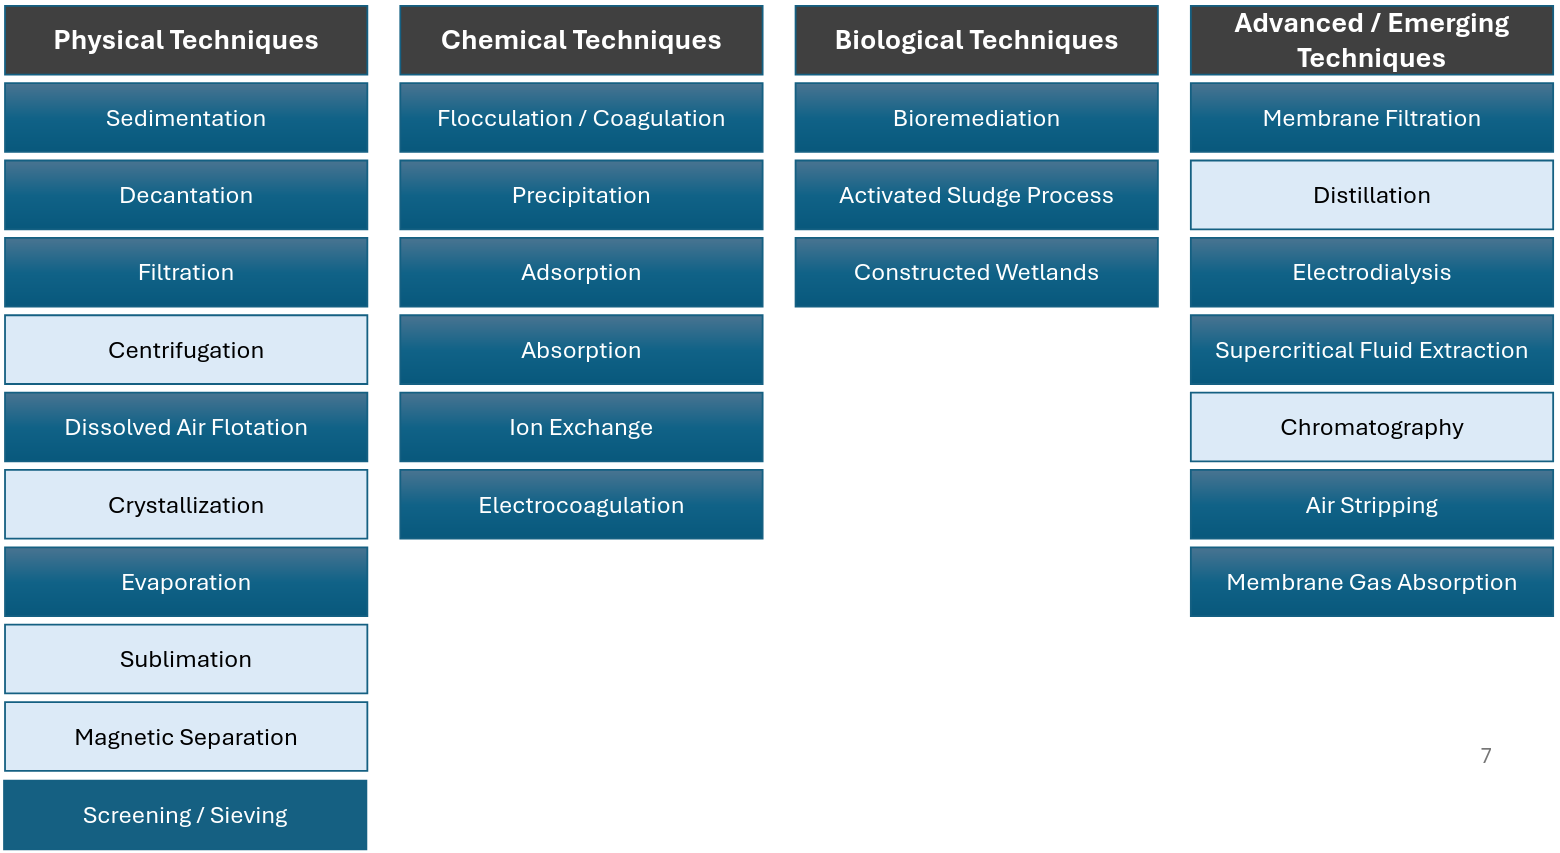
\includegraphics[width=\textwidth]{media/techniques_overview.png}
    \caption*{Separation techniques overview}
\end{figure*}

\section{Physical separation}
\subsection{Sedimentation}

\subsection{Decantation}

\subsection{Filtration}

\subsubsection{Sand filtration}

\subsubsection{Reverse osmosis}

\subsection{Centrifugation}

\subsection{Dissolved Air Flotation (DAF)}

\subsection{Magnetic separation}

\subsection{Screening and Sieving}

\newpage
\section{Chemical separation}

\subsection{Flocculation}
\subsubsection{Flocculant}

\subsubsection{Coagulation}

\subsection{Electrocoagulation}

\subsection{Precipitation}

\subsection{Adsorbtion}

\subsubsection{Activated carbon}

\subsection{Absorption}

\subsubsection{Wet scrubber}

\subsection{Ion exchange}

\subsection{Crystallization}

\subsection{Evaporation}

\subsection{Sublimation}

\newpage
\section{Advanced/Emerging separation}

\subsection{Mebrane filtration}

\subsubsection{Micro osmosis}

\subsubsection{Nano osmosis}

\subsubsection{Ultra osmosis}

\subsubsection{Reverse osmosis}

\subsection{Electrodialysis}

\subsection{Extraction}

\subsubsection{Liquid-Liquid Extraction (LLE)}

\subsubsection{Soxhlet extraction}

\subsubsection{Supercritical Fluid Extraction}

\subsection{Air stripping}
Same as Wet Scrubber, but with water

\subsection{Electrostatic precipitator (ESP)}

\newpage
\section{Biological separation}
\subsection{Bioremediation}
\begin{itemize}
    \item Miicroorganisms degrade hazardous substances
    \item Useful for oil spills, soil remediation
\end{itemize}

\subsection{Activated Sludge Process}
\begin{itemize}
    \item Aerobic digestion of organic matter
    \item Common in sewage treatment
    \item A parameter to monitor is the BOD (Biochemical Oxygen Demand) and COD (Chemical Oxygen Demand)
    \item Nitrification and Denitrification
\end{itemize}

\subsection{Constructed Wetlands}
\begin{itemize}
    \item Mimics natural wetlands to treat wastewater
    \item Sustainable and low-maintenance
    \item Three types
    \item It takes 1-4 weeks to treat the water
\end{itemize}

\part{Ecological sanitation}
\dots

\section{Some principles of Sanitation}

\section{Objectives of ecological sanitation}
\begin{itemize}
    \item Provide affordable, hygenically safe, and desirable sanitary facilites
    \item Reduce the health risks related to sanitation, contaminated water an waste
    \item Prevent the pollution of surface and groundwater; precenti the degradation of soil fertility
    \item Optimise the management of nutrients and water resources
\end{itemize}

\section{Principle of treatments and recycling}

\section{Wastewater management}
\subsection{Issues with current wastewater management (Linear End-of-Pipe Technology)}
\subsubsection{Poor treatment or uncontrolled discharge}

\subsubsection{High water use}

\subsubsection{Costly systems}

\subsubsection{Unequal service}

\subsubsection{Resource loss}

\subsubsection{Sewage sludge issues}

\subsection{Benefits of Material Flow Cycle (Instead of Disposal)}
\subsubsection{Better health}

\subsubsection{Resource recovery}

\subsubsection{Soil and crop benefits}

\subsubsection{Resource efficiency}

\subsubsection{Smarter systems}

\subsubsection{Holistic approach}

\section{Separation of substances}
\begin{figure*}[ht!]
    \centering
    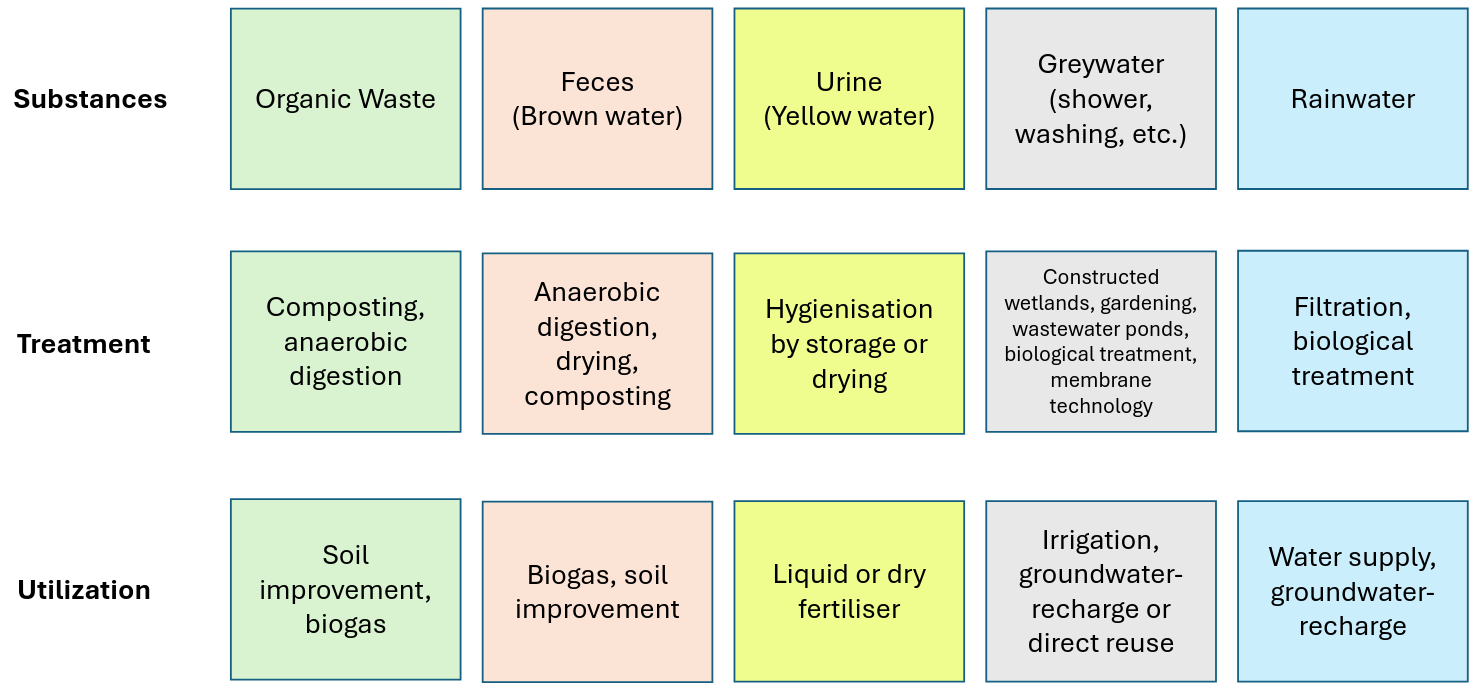
\includegraphics[width=\textwidth]{media/separation_of_substances.png}
\end{figure*}


















\end{document}
